% !TeX program = pdflatex
\documentclass[border=6pt]{standalone}
\usepackage{tikz}
\usetikzlibrary{arrows.meta, positioning, calc}

\definecolor{MediumRed}{rgb}{0.925, 0.345, 0.345}
\definecolor{MediumGreen}{rgb}{0.37, 0.7, 0.66}
\definecolor{MediumBlue}{rgb}{0.015, 0.315, 0.45}
\definecolor{DarkBlue}{rgb}{0.05, 0.15, 0.35}

\newcommand{\card}[6]{% x, y, borde, titulo, cuerpo, cifra
    \node[draw=#3, very thick, rounded corners=6pt, fill=#3!8, text=DarkBlue,
          align=left, text width=6.0cm, minimum height=2.6cm, anchor=north west,
          font=\sffamily\footnotesize] at (#1,#2)
        {\textbf{\textcolor{#3!70!black}{#4}}\\[3pt]#5\\[4pt]{\normalsize\bfseries\textcolor{#3!70!black}{#6}}};
}

\begin{document}
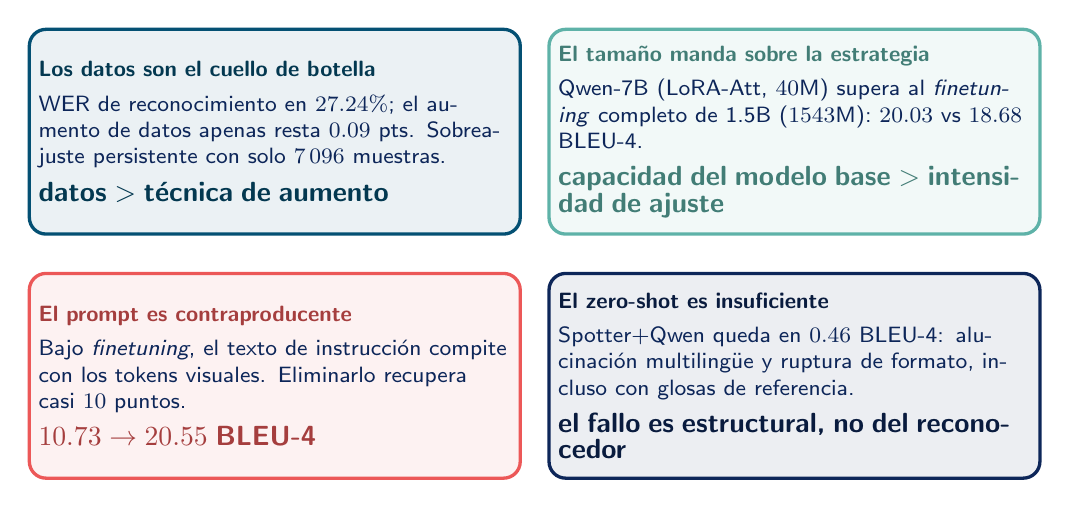
\begin{tikzpicture}[font=\sffamily]

\card{0}{0}{MediumBlue}{Los datos son el cuello de botella}
    {WER de reconocimiento en $27.24\%$; el aumento de datos apenas resta $0.09$~pts. Sobreajuste persistente con solo $7\,096$ muestras.}
    {datos $>$ técnica de aumento}

\card{6.6}{0}{MediumGreen}{El tamaño manda sobre la estrategia}
    {Qwen-7B (LoRA-Att, $40$M) supera al \textit{finetuning} completo de 1.5B ($1543$M): $20.03$ vs $18.68$ BLEU-4.}
    {capacidad del modelo base $>$ intensidad de ajuste}

\card{0}{-3.1}{MediumRed}{El \textit{prompt} es contraproducente}
    {Bajo \textit{finetuning}, el texto de instrucción compite con los tokens visuales. Eliminarlo recupera casi $10$ puntos.}
    {$10.73 \rightarrow 20.55$ BLEU-4}

\card{6.6}{-3.1}{DarkBlue}{El \textit{zero-shot} es insuficiente}
    {Spotter+Qwen queda en $0.46$ BLEU-4: alucinación multilingüe y ruptura de formato, incluso con glosas de referencia.}
    {el fallo es estructural, no del reconocedor}

\end{tikzpicture}
\end{document}
